\chapter[Desenvolvimento]{Desenvolvimento}
\label{cap:desenvolvimento}

Após o planejamento do projeto, foi feito o desenvolvimento de cada etapa.
Inicialmente, foi feito o desenvolvimento da placa de controle para poder acionar os motores.
Em seguida, o \textit{software} para ler os dados das manetes e enviar os comandos para a placa de controle foi desenvolvido.

\section[Desenvolvimento da placa de controle]{Desenvolvimento da placa de controle}
\label{sec:desenvolvimentoPlacaControle}

Primeiramente, foi feito o desenvolvimento da placa de controle dos manipuladores, pois é necessária para testar o funcionamento dos motores e do \textit{software} que será desenvolvido.
Para isso, foi necessário definir quais componentes utilizar e como conectá-los.

Conforme descrito na subseção \ref{sub:placaControle}, a placa de controle deve utilizar uma ponte H para o controle de cada junta.
Para isso, foi escolhido o CI L293D, que possui duas pontes H e suporta tensões de 12V.
Como é necessário controlar 6 motores, foram utilizados 3 CI L293D.

Para simplificar o controle e evitar problemas de acionamento duplo das entradas das pontes H, foi utilizado o CI 74LS02 como um inversor lógico.
Dessa forma, a placa de controle possui para cada junta uma entrada de \textit{Enable} para ligar/desligar o acionamento da junta, e uma porta de \textit{Direction} para definir a direção de movimentação dela.
A partir dessas entradas, o CI L293D é acionado e o motor é controlado.
A Figura \ref{fig:esquematicoSimplificado} mostra o esquemático simplificado de um CI L293D e um CI 74LS02.

\begin{figure}[H]
    \centering
    \caption{Esquemático Simplificado de um CI L293D e um CI 74LS02}
    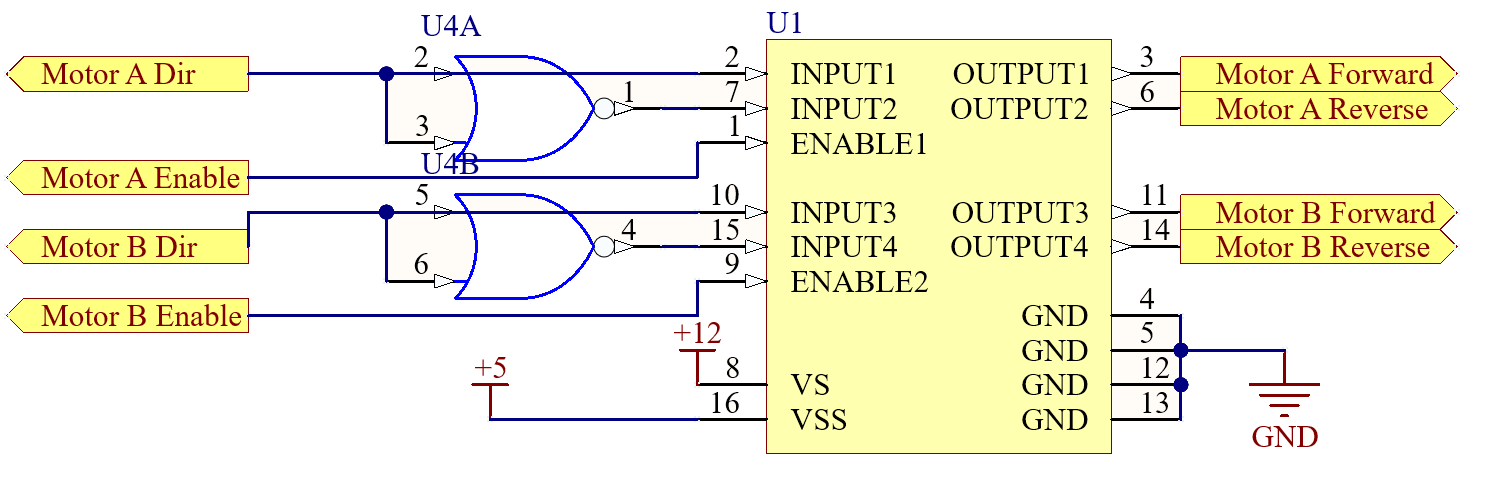
\includegraphics[keepaspectratio=true, width=0.9\textwidth]
    	{img/placa-controle-esquematico-simplificado.png}
    \fonte{Do próprio autor}
    \label{fig:esquematicoSimplificado}
\end{figure}

Com os componentes principais definidos foi feito o desenvolvimento do esquemático da placa de controle com o auxílio do software \textit{Altium Designer}.
O Anexo \ref{anexo:esquematico-placa-controle} mostra o esquemático completo da placa de controle.
Nesse esquemático foram adicionados resistores de \textit{pulldown} para garantir que as entradas dos CI L293D e 74LS02 permaneçam em nível lógico baixo caso não estejam conectadas ao microcontrolador.
Também foram adicionadas \textit{LEDs} para indicar a alimentação de 5V e 12V da placa.

Após o desenvolvimento do esquemático, foi feita a montagem da Placa de Circuito Impresso (PCB), ainda com o auxílio do software \textit{Altium Designer}.
Para isso, os componentes foram posicionados no \textit{layout} da placa, tendo em vista a economia de espaço e a necessidade de manter os componentes próximos para facilitar sua conexão.
Em seguida, as trilhas e vias que realizam a conexão dos componentes foram desenhadas. 
Para permitir a conexão de todos os componentes, foi necessário utilizar uma placa com 2 camadas.
A Figura \ref{fig:placaControleLayout} mostra o \textit{layout} final da placa de controle.

Com o \textit{layout} finalizado, foi feita a produção da PCB de forma manual.
Para isso, o negativo do \textit{layout} foi impresso em uma folha de transparência.
Depois, uma placa de circuito impresso de duas camadas foi cortada no tamanho desejado.

Em seguida, foi feita a transferência do \textit{layout} para a placa.
Para isso, uma fina camada de tinta fotossensível destinada para PCB foi aplicada sobre a placa.
Essa tinta foi pré-curada à 75$^{\circ}$C durante 15 minutos com o auxílio de uma base de aquecimento, para garantir que ela não se descolasse da placa.
Após a pré-cura, a tinta foi exposta à luz ultravioleta por 3 minutos, utilizando a transparência com o \textit{layout} como máscara.
Em seguida, a placa foi submersa em uma solução de carbonato de sódio para realizar a revelação do \textit{layout}.
Após a placa ser revelada, a tinta foi curada à 85$^{\circ}$C durante 30 minutos.

Esse processo de transferência do \textit{layout} foi repetido para a segunda camada da placa.
Em seguida, foi utilizada uma solução de percloreto de ferro para corroer as áreas de cobre que não receberam tinta.
Após a corrosão, a placa foi mergulhada em uma solução de hidróxido de sódio para remover a tinta.

Após a corrosão da PCB, foi feita a perfuração das vias e dos furos para os componentes.
Por fim, foi feita a soldagem dos componentes na placa e a conexão das vias.
A Figura \ref{fig:placaControle} mostra a placa de controle montada.

\begin{figure}[H]
    \begin{minipage}{.5\textwidth}
        \centering
        \caption{Layout da placa de controle}
        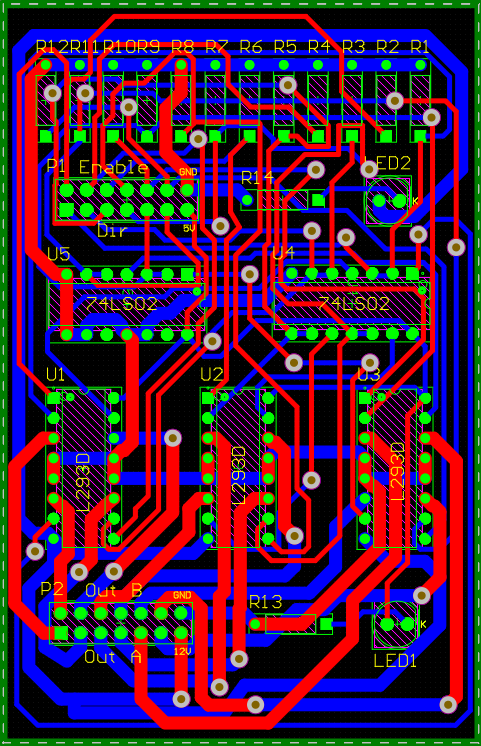
\includegraphics[keepaspectratio=true, width=0.9\linewidth]
            {img/placa-controle-layout.png}
        \fonte{Do próprio autor}
        \label{fig:placaControleLayout}
    \end{minipage}%
    \begin{minipage}{.5\textwidth}
        \centering
        \caption{Placa de controle produzida}
        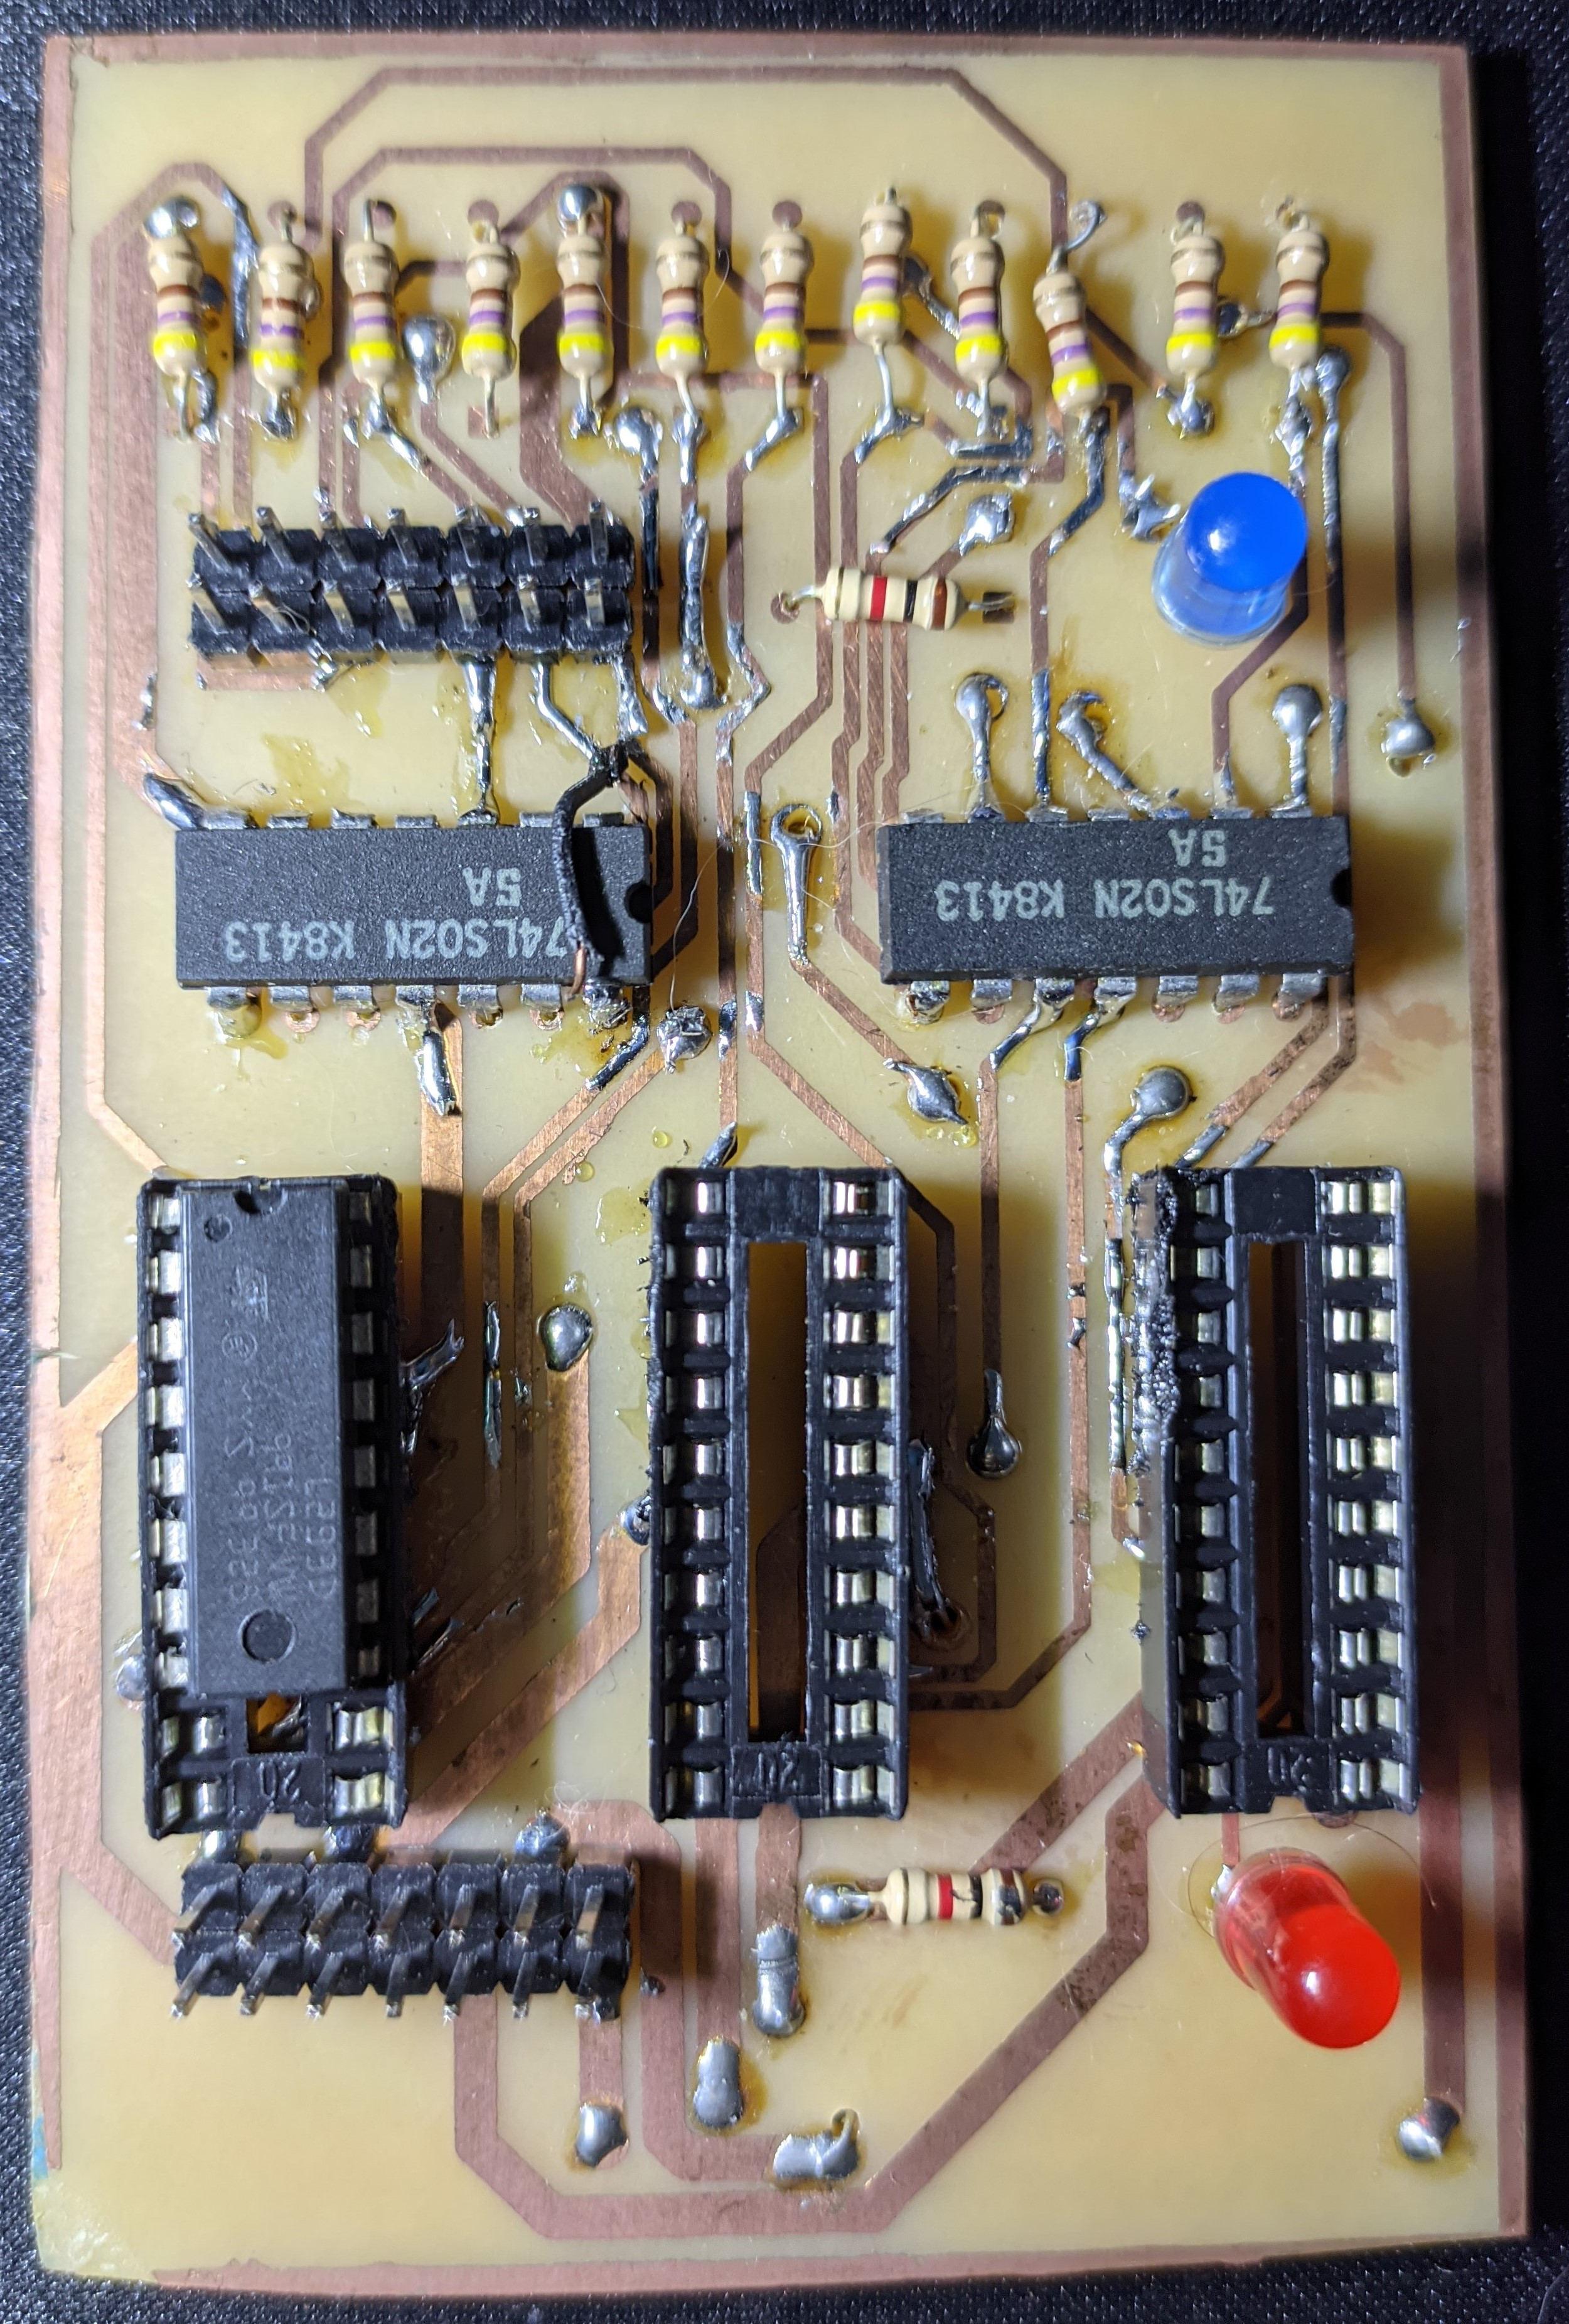
\includegraphics[keepaspectratio=true, width=0.9\linewidth]
            {img/placa-controle.jpg}
        \fonte{Do próprio autor}
        \label{fig:placaControle}
    \end{minipage}%    
\end{figure}

\section[Leitura das manetes]{Leitura das manetes}
\label{sec:leituraManetes}

Após a montagem da placa de controle, foi desenvolvido um \textit{software} com o microcontrolador para realizar a leitura dos dados das manetes.
Conforme descrito na subseção \ref{sub:maneteJogadores}, cada manete possui dois \textit{joysticks} com dois eixos e um botão cada.

Para realizar a leitura dos eixos dos \textit{joysticks}, foram utilizadas as entradas analógicas do microcontrolador.
Como o Arduino utiliza um conversor analógico-digital de 10 bits, os valores lidos variam de 0 a 1023.
Valores próximos de 512 representam a posição central do \textit{joystick}, enquanto valores próximos de 0 ou 1023 representam as posições extremas.
Para aprimorar a usabilidade da manete, foi implementada uma área de \textit{deadzone}, na qual o valor lido é considerado como zero, para evitar que o manipulador se movimente sem a intenção do usuário.

Para realizar a leitura do botão, foi utilizada uma entrada digital.
Esses botões possuem um \textit{pull-up} interno, o que significa que o valor lido é 1 quando o botão não está pressionado e 0 quando o botão está pressionado.

Os valores lidos são armazenados em uma variável, que é utilizada para realizar o controle do movimento do manipulador robótico.

\section[Cálculo da posição]{Cálculo da posição}
\label{sec:calculoPosicao}

Para calcular a posição do manipulador robótico, foi utilizado como base o \textit{software} desenvolvido anteriormente para ler os dados das manetes.

Para essa primeira parte do trabalho, o cálculo de posição foi feito de forma individual para cada junta.
Dessa forma, o usuário pode utilizar os 4 eixos dos \textit{joysticks} para controlar o manipulador robótico.
Além disso, o usuário pode utilizar o botão de cada manete para controlar a abertura e o fechamento da garra.

\section[Controle dos motores]{Controle dos motores}
\label{sec:controleMotores}

O controle dos motores foi incorporado no \textit{software} desenvolvido na subseção anterior, que realiza o cálculo da posição desejada das juntas.

Primeiramente foi implementada a leitura da posição atual de cada junta, utilizando as entradas analógicas do microcontrolador.
Os valores de 10 bits lidos pelo Arduino são convertidos para graus, utilizando como referência as faixas de movimento descritas nas tabelas \ref{tab:caracteristicasManipuladorMentor} e \ref{tab:caracteristicasManipuladorAzul}.

Depois disso, foi feita a implementação de um controlador para o manipulador.
Esse controlador é executado a cada 10ms, de acordo com a configuração da interrupção do \textit{timer} do Arduino.
Nessa interrupção, o microcontrolador calcula o erro entre a posição desejada e a posição atual de cada junta, com base nos valores lidos do manipulador e das manetes.
Em seguida, o valor de saída é calculado utilizando um algoritmo PID.
Esse algoritmo utiliza três constantes (Kp, Ki e Kd) e os valores do erro atual, da integral dos erros anteriores e da derivada do erro atual para calcular a saída.
Por fim, esse valor de saída é convertido em um valor de \textit{duty cycle}, e é utilizado para gerar o sinal PWM enviado para a placa de controle.